\title[Daten Vorhersagen]{Daten Vorhersagen}
\date{\today}
\subtitle{PageRank}
\logo{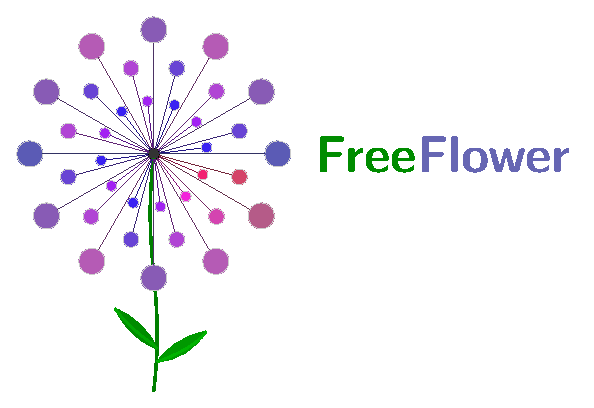
\includegraphics[width=.7cm]{Logos/FreeFlower.pdf}}

\frame{\titlepage}

\section{PageRank}

\begin{frame}{Themenübersicht}
    \begin{columns}
        \column{0.48\textwidth}
        \begin{figure}[H]
            \centering
            \begin{tikzpicture}[node distance=2.1cm, thick, >=stealth']
                \tikzset{site/.style={circle, draw, minimum size=10mm, font=\small\bfseries}}
                \node[site] (A) at (0,1.2) {A};
                \node[site] (B) at (2.3,1.2) {B};
                \node[site] (C) at (1.15,-0.7) {C};
                \node[site] (D) at (3.4,-0.7) {D};
                \path[->] (A) edge[bend left=18] (B)
                (A) edge[bend right=12] (C)
                (B) edge (C)
                (C) edge[bend left=18] (A)
                (D) edge (C);
            \end{tikzpicture}
            \caption*{Netzwerk mit 4 Seiten}
        \end{figure}
        \column{0.48\textwidth}
        \begin{itemize}
            \item[\faSquare] Zufälliger Surfer
            \item[\faSquare] Dämpfungsfaktor $d=0.85$
            \item[\faSquare] Iteration bis Stabilität
            \item[\faSquare] Manipulation / Bias
        \end{itemize}
    \end{columns}
\end{frame}

\begin{frame}{Grundidee}
    \begin{columns}
        \column{0.54\textwidth}
        \begin{figure}[H]
            \centering
            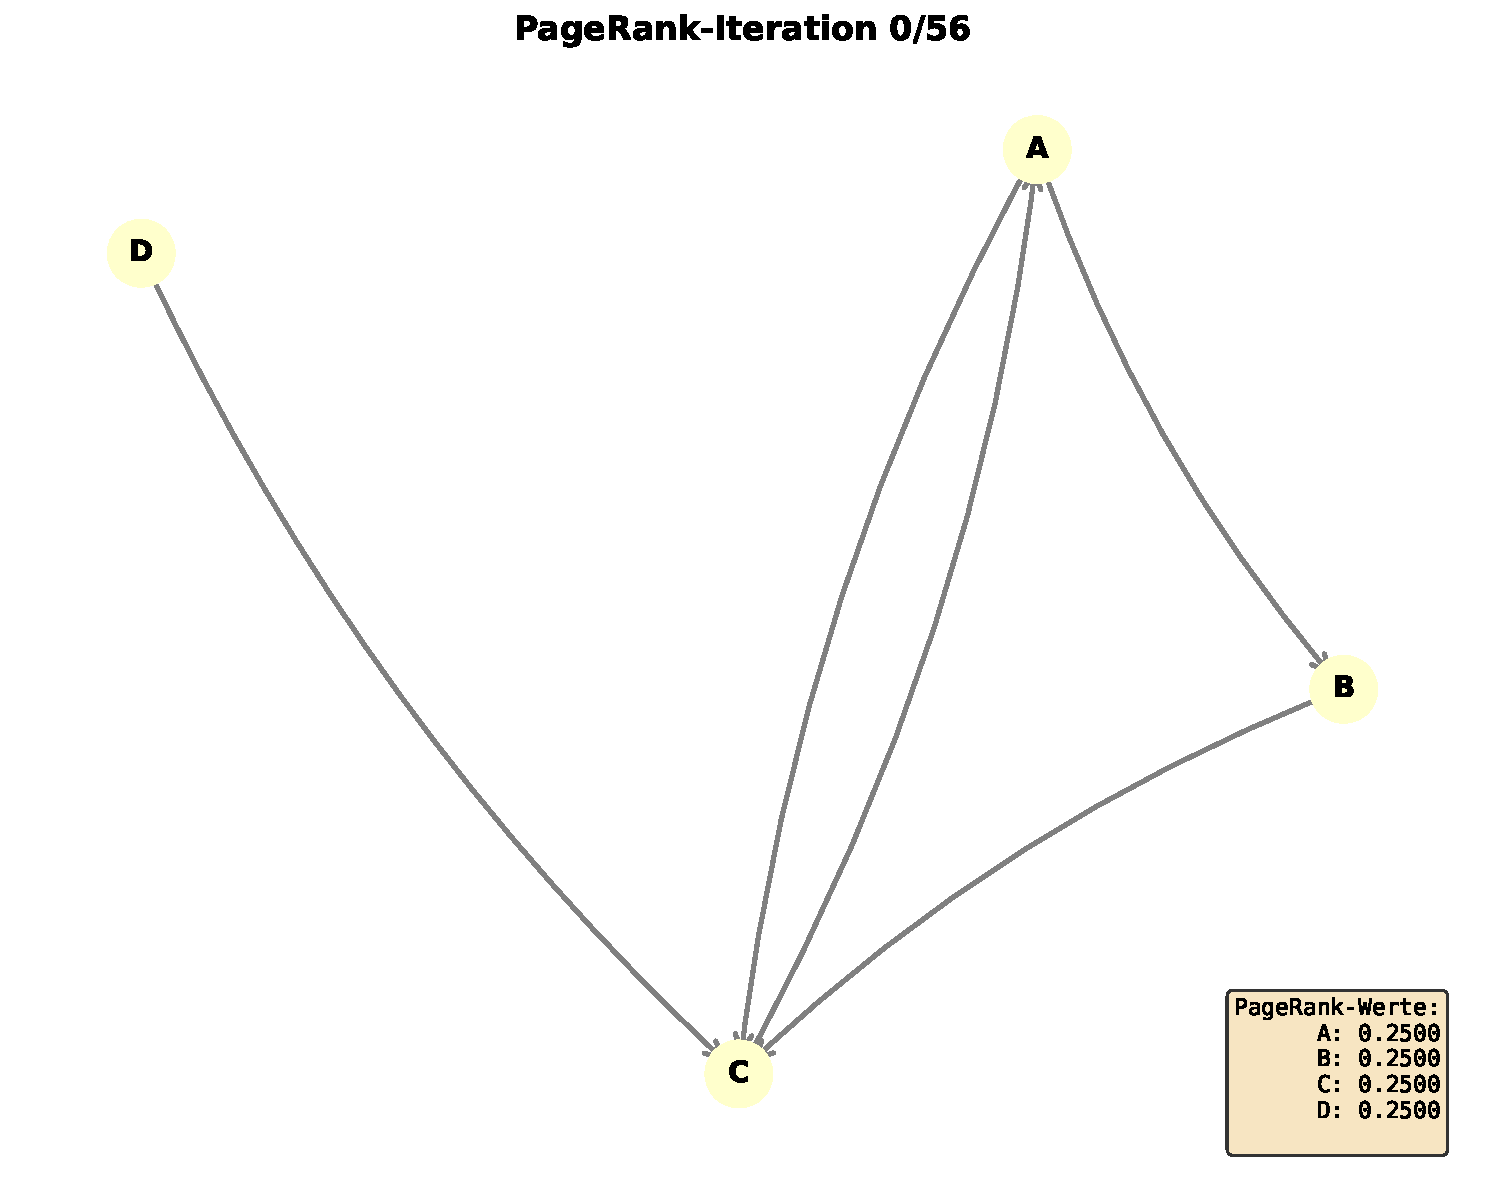
\includegraphics[width=\linewidth]{Grundlagen_Info/10_KI_und_Algorithmen/Figures/pagerank_step_00.pdf}
            \caption*{Startwerte: alle Seiten gleich wichtig}
        \end{figure}
        \column{0.42\textwidth}
        \begin{mydefinition}[PageRank]
            Wichtig ist nicht nur die Anzahl der Links, sondern auch deren \textbf{Qualität}.
        \end{mydefinition}
        \vspace{0.4em}
    \end{columns}
    \[PR(p)=\frac{1-d}{N}+d\sum_{q\to p}\frac{PR(q)}{\mathrm{outdeg}(q)}\]
    \vspace{0.4em}
    \begin{center}
        \large \(d=0.85\), \(\frac{1-d}{N}=0.0375\)
    \end{center}
\end{frame}

\begin{frame}{Ein Schritt}
    \[
        \begin{array}{c|cccc|c}
              & A & B & C & D & \text{outdeg} \\
            \hline
            A & 0 & 1 & 1 & 0 & 2             \\
            B & 0 & 0 & 1 & 0 & 1             \\
            C & 1 & 0 & 0 & 0 & 1             \\
            D & 0 & 0 & 1 & 0 & 1             \\
        \end{array}
    \]
    \begin{myexample}
        Start: \(PR(A)=PR(B)=PR(C)=PR(D)=0.25\)
        \[
            \begin{aligned}
                PR(A) & = 0.0375 + 0.85\cdot 0.25 = \underline{0.25000}  \\
                PR(B) & = 0.0375 + 0.85\cdot 0.125 = \underline{0.14375} \\
                PR(C) & = 0.0375 + 0.85\cdot 0.625 = \underline{0.56875} \\
                PR(D) & = \underline{0.0375}
            \end{aligned}
        \]
    \end{myexample}
\end{frame}

\foreach \step in {00,01,02,03,04,05}{
        \begin{frame}{Iteration \step}
            \begin{figure}[H]
                \centering
                \includegraphics[width=\linewidth]{Grundlagen_Info/10_KI_und_Algorithmen/Figures/pagerank_step_\step.pdf}
                \caption*{Schritt \step}
            \end{figure}
        \end{frame}
    }

\begin{frame}{Finale Werte}
    \begin{columns}
        \column{0.6\textwidth}
        \begin{figure}[H]
            \centering
            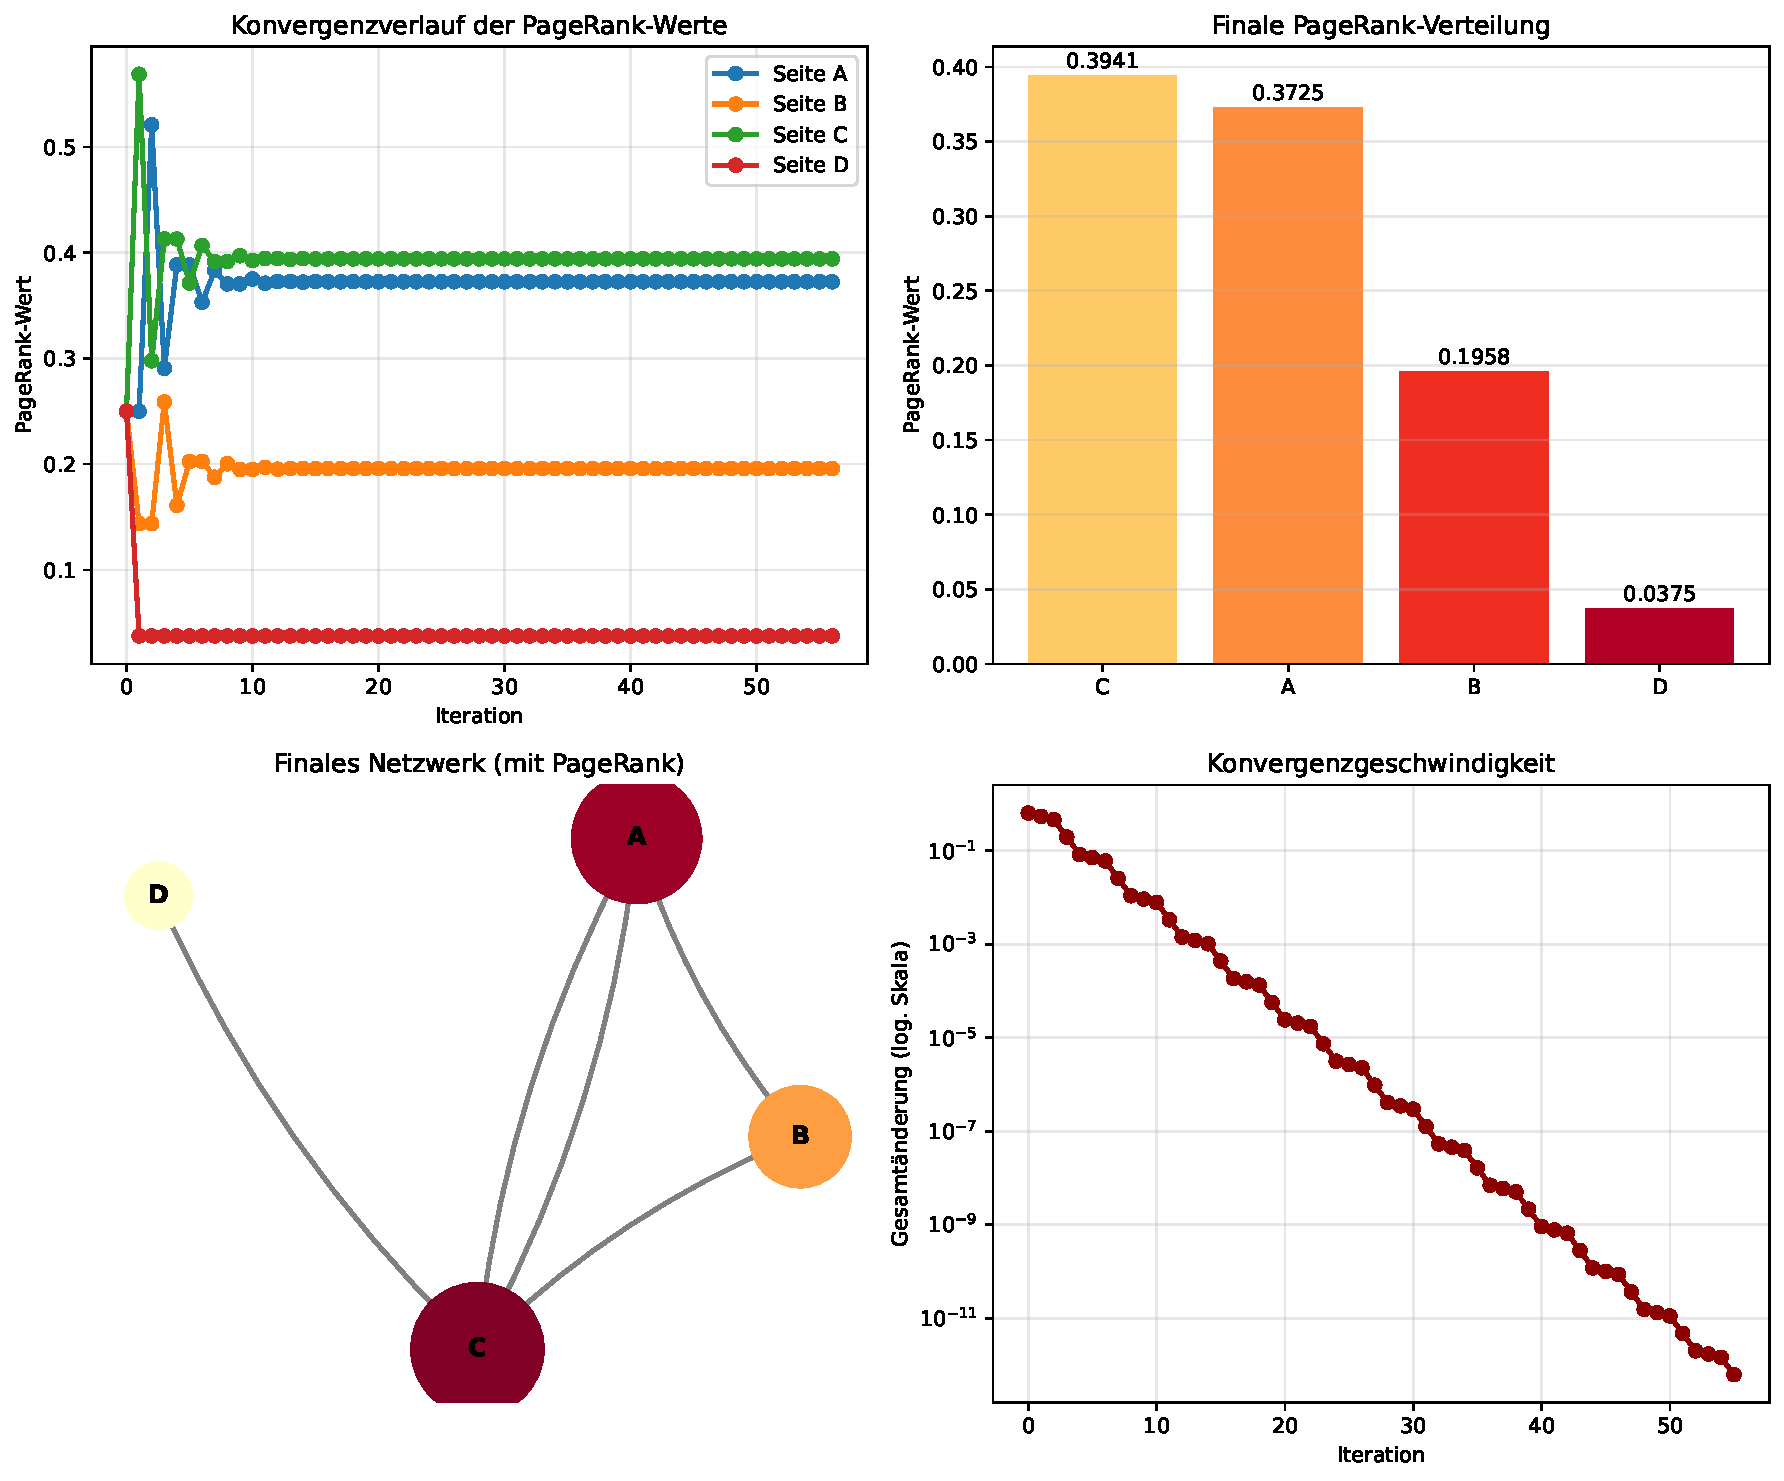
\includegraphics[width=\linewidth]{Grundlagen_Info/10_KI_und_Algorithmen/Figures/pagerank_summary.pdf}
            \caption*{Endstand nach Konvergenz}
        \end{figure}
        \column{0.38\textwidth}
        \begin{table}[H]
            \centering
            \begin{tabular}{c|c}
                Seite & PR      \\
                \hline
                C     & 0.56875 \\
                A     & 0.25000 \\
                B     & 0.14375 \\
                D     & 0.03750 \\
            \end{tabular}
        \end{table}
        \vspace{0.7em}
        \begin{center}
            \large Höchster Wert: \textbf{C}
        \end{center}
    \end{columns}
\end{frame}

\begin{frame}{Intuitives Lesen}
    \begin{columns}
        \column{0.55\textwidth}
        \begin{myexercise}[PageRank intuitiv lesen]
            \begin{itemize}
                \item A \(\to\) B, C
                \item B \(\to\) C
                \item C \(\to\) A
                \item D \(\to\) C
            \end{itemize}
        \end{myexercise}
        \column{0.4\textwidth}
        \begin{myanswer}
            C ist nach einem Schritt am stärksten.

            Ein Link von einer Seite mit vielen Ausgängen zählt weniger, weil sich der Score auf mehrere Ziele verteilt.
        \end{myanswer}
    \end{columns}
\end{frame}

\begin{frame}{Manipulation}
    \begin{columns}
        \column{0.5\textwidth}
        \begin{mycaution}
            Linkfarmen, gekaufte Links und starke Netzwerke können die Rangfolge verzerren.
        \end{mycaution}
        \column{0.44\textwidth}
        \begin{figure}[H]
            \centering
            \begin{tikzpicture}[node distance=1.7cm, thick, >=stealth']
                \tikzset{n/.style={circle, draw, minimum size=9mm, font=\small\bfseries, fill=gray!10}}
                \node[n] (L1) at (0,1.1) {L1};
                \node[n] (L2) at (1.8,1.1) {L2};
                \node[n] (L3) at (0.9,-0.2) {L3};
                \path[->] (L1) edge[bend left=12] (L2)
                (L2) edge[bend left=12] (L3)
                (L3) edge[bend left=12] (L1)
                (L1) edge[bend right=12] (L3)
                (L2) edge[bend right=12] (L1);
            \end{tikzpicture}
            \caption*{Geschlossene Linkgruppe}
        \end{figure}
    \end{columns}
\end{frame}

\begin{frame}{Notebook}
    \begin{columns}
        \column{0.55\textwidth}
        \begin{myremark}[Praktische Umsetzung]
            \href{https://cyrilblum.github.io/FreeFlower/jupyter/}{\texttt{10\_KI\_und\_Algorithmen/06\_Priorisierung\_PageRank.ipynb}}
        \end{myremark}
        \column{0.4\textwidth}
        \begin{figure}[H]
            \centering
            % \includegraphics[width=\linewidth]{Grundlagen_Info/10_KI_und_Algorithmen/Figures/pagerank_animation.gif}
            \caption*{Animation der Iterationen}
        \end{figure}
    \end{columns}
\end{frame}

\begin{frame}{Kurzfazit}
    \begin{center}
        \Large Wichtig ist nicht nur \enquote{wie viele}, sondern \enquote{von wem}.
    \end{center}
\end{frame}
